\documentclass[a4paper,11pt]{article}
\usepackage[spanish]{babel}
\usepackage[utf8]{inputenc}

% Configuración páginas
\usepackage{vmargin}				% Márgenes

\usepackage{sectsty}				% Fuente de los títulos
\allsectionsfont{\normalfont \Large \scshape}

\usepackage{graphicx}				% Imágenes
\graphicspath{{images/}}

\usepackage{listliketab}			% Tratar indentación de listas como tablas

\usepackage{mathtools}				% Matematicas
\newcommand\numberthis{				% numeración en align*
	\addtocounter{equation}{1}\tag{\theequation}
}

% Configuración del título
\newcommand{\horrule}[1]{\rule{\linewidth}{#1}} 	% Horizontal rule

\title{
	\vspace{-25pt}
	\normalfont \Large \textsc{
		Modelos de Investigación Operativa,
        Ingeniería Informática\\
        Universidad de Valladolid
	}\\[10pt]
	\horrule{1pt}\\[10pt]
	\huge \textbf{
		Práctica 6
	}\\
	\horrule{1pt}
}
\author{
	\normalfont \Large Daniel González Alonso
}
\date{
	\normalfont \large \today
}

%%%%%%%%%%%%%%%%%%%%%%%%%%%%%%%%%%%%%%%%%%%%%%%%%%
\begin{document}
\maketitle

%%%% RESUMEN %%%%
\begin{abstract}
	En este documento se describen los problemas y los resultados obtenidos de la práctica 6 del tema 3 de la asignatura Modelos de Investigación Operativa de Ingeniería Informática, Universidad de Valladolid.
\end{abstract}

%%%% DESARROLLO %%%%
\section{Introducción}
%%%%%%%%%%%%%%%%%%%%%%%%%%%%%%%%%%%%%%%%%%%%%%%%%%%%%%
Esta práctica trataba de problemas de Set Covering. El modelo empleado para resolver los problemas de Set Covering es el siguiente:

\begin{align*}\numberthis
   	&\textrm{Minimizar }	&& \sum_{j=1}^{n}{f_j \cdot x_j} \\
   	&\textrm{Sujeto a }		&& \sum_{j \in N_{i}}{a_{i,j} \cdot x_{j} \geq 1} 	&& i=1,\ldots,m \\
	&						&& x_{j} \in \{0,1\}					&& j=1,\ldots,n
\end{align*}

Donde ${m}$ es el número de puntos de demanda, ${n}$ es el número de posibles puntos de servicio, ${f_j}$ representa el coste de instalar un punto de servicio en ${j}$ y la matriz ${a_{i,j}}$ contiene solo los valores 1 si ${i}$ está cubierto por ${j}$ o 0 en caso contrario.\\

\newpage
\section{Ejercicios}

\subsection{Práctica 6.1}
Para esta práctica se nos pide resolver el problema de los condados de Nueva York (conjunto de datos \texttt{data/matriz30x30.dat}) con el método greedy para valores de la distancia de cubrimiento entre 70 y 120, y comparar los resultados con los obtenidos de forma óptima con Xpress.\\

Este problema se encuentra resuelto mediante \textit{Xpress Mosel} en el archivo \texttt{set\_covering\_6\_1.mos}. Lo primero que hicimos en el archivo fue cargar los datos del fichero de datos, en la primera linea del archivo venía dado el valor de ${m}$, en la segunda el valor de ${n}$ y en los siguientes la matriz de distancias ${d_{i,j}}$.\\

A continuación se creó un bucle que iteraba entre los valores de ${dc}$ pedidos. En cada iteración lo primero que se hace es calcular la matriz ${a_{i,j}}$ mediante la distancia de cubrimiento ${dc}$ actual y la matriz de distancias ${d_{i,j}}$. Lo siguiente es calcular la solución exacta mediante \textit{Xpress} y el modelo presentado anteriormente, finalmente en cada iteración también se calcula la solución mediante el método greedy, el cual se describe a continuación:

\begin{enumerate}
\item Calcular el número de puntos de demanda no cubiertos que cubre cada posible punto de servicio que todavía no se encuentra en la solución. En mi caso lo almacené en un vector llamado ${d_{j}}$, y solo lo calculaba para todos aquellos posibles puntos de servicio que no se encontraran marcados en otro vector llamado \texttt{fijadas}. Además tengo otro vector llamado \texttt{cubiertas} para saber que punto de demanda ya está cubierto y quien no.
\item Buscamos el elemento que minimiza el criterio greedy ${\frac{c_{j}}{d_{j}}}$. Como para este problema los valores de coste ${c_{j}}$ no se nos da, suponemos un valor 1 (minimizamos el número d instalaciones). A este elemento le llame en el código como \texttt{j\_min}.
\item Añadimos \texttt{j\_min} a la solución. Además en mi caso la añado al vector con elementos fijados.
\item Marcamos los puntos de demanda cubiertos por \texttt{j\_min} como ya cubiertos.
\item En caso de que el número de puntos de servicio instalados se menor que ${m}$ volvemos al paso 1, si no ya hemos alcanzado la solución Greedy.
\end{enumerate}

La evolución de los resultados obtenidos con los distintos valores de ${dc}$ se pueden observar en la siguiente gráfica, la cual compara los resultados de la solución exacta y la del algoritmo greedy:

\begin{figure}[!htbp]
	\centering
	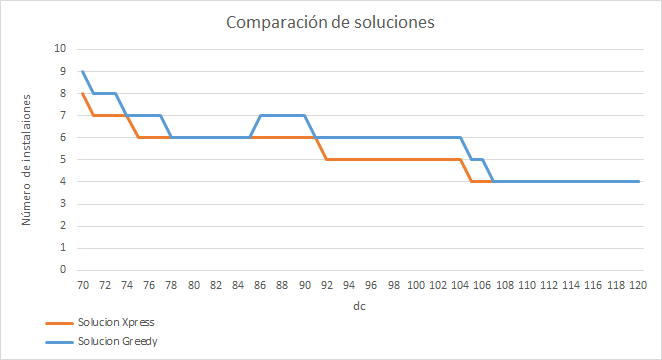
\includegraphics[width=0.9\textwidth]{6_1_comparacion.png}
    \caption{Comparación de los resultados de la solución de Xpress y el Método Greedy para la práctica 6.1}
\end{figure}

\newpage
\subsection{Práctica 6.2}
Para la práctica 6.2 se nos pide resolver los problemas \texttt{aint1.dat} y \texttt{aint5.dat} para ${dc}$ desde 250 hasta 400, con los métodos greedy, greedy aleatorizado (para ${K=5}$ y ${N=100}$), y comparar con el método exacto.\\

Esta práctica se encuentra resuelta mediante \textit{Xpress Mosel} en los archivos \texttt{set\_covering \_6\_2\_aint1.mos} y \texttt{set\_covering\_6\_2\_aint5.mos}. En ambos ficheros los primero que se hizo fue cargar los datos. Los datos de los ficheros \textit{aint} vienen dados de la siguiente forma:

\storestyleof{itemize}
\begin{listliketab}
    \begin{tabular}{Lll}
\textbullet	& ${m}$							& Número de puntos de demanda	\\
\textbullet	& ${n}$ 						& Número de puntos de servicio	\\
\textbullet	& ${h_i		\ \ i=1,\ldots,m}$	& Demandas, una por línea		\\
\textbullet	& ${d_{i,j}	\ \ i=1,\ldots,m \ \ j=1,\ldots,n}$	& Matriz ${m \times n}$ de distancias (Hectómetros)	\\
    \end{tabular}
\end{listliketab}

A continuación se creó un bucle que iteraba entre los valores de ${dc}$ pedidos.  En cada iteración se obtiene el resultado para el método exacto, el método greedy y el método greedy aleatorizado. Como el método exacto y el greedy ya se ha explicado (la única diferencia en este problema tiene que ver con que para este problema si disponemos de los costes ${c_{j}}$), procederé a explicar el Método Greedy Aleatorizado.\\

En el método Greedy Aleatorizado a diferencia del Greedy normal disponemos de una lista \textit{RCL} donde introduciremos los ${K}$ indices (5 en nuestro caso) con los mejores valores para el criterio Greedy en la iteración actual, y de entre ellos se selecciona uno aleatoriamente para así obtener el elemento \texttt{j\_min}. En mi caso para hacer esta parte
cree un vector para la lista \textit{RCL} de tamaño ${K}$ y otro llamado \texttt{marcadas} que sirve para indicar si un elemento ya se encuentra en la lista \textit{RCL} o no el cual reiniciaba en cada iteración. Este cálculo se hace de forma idéntica a la del algoritmo Greedy con la única diferencia de que hay que tener en cuenta si un elemento ya se encuentra en la lista o no. Por otro lado, otra de las diferencias de este método es que estos pasos anteriores tienen que ejecutarse ${N}$ veces (en nuestro caso 100), y en cada una de las iteraciones se comprueba si la solución obtenida es mejor que la de las iteraciones anteriores.\\

Las soluciones obtenidas para los ficheros de datos \texttt{aint1.dat} y \texttt{aint5.dat} se muestran a continuación:

\begin{figure}[!htbp]
	\centering
	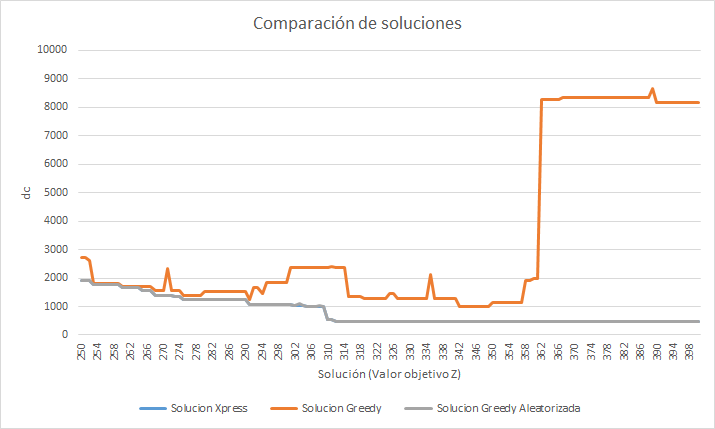
\includegraphics[width=0.9\textwidth]{6_2_aint1_comparacion.png}
    \caption{Comparación de los resultados para el archivo de datos \texttt{aint1}}
\end{figure}

\begin{figure}[!htbp]
	\centering
	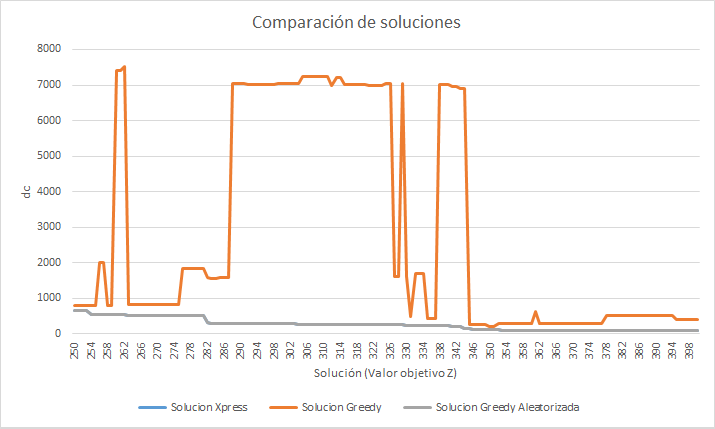
\includegraphics[width=0.9\textwidth]{6_2_aint5_comparacion.png}
    \caption{Comparación de los resultados para el archivo de datos \texttt{aint5}}
\end{figure}

\end{document}
